\section{Metodi}
VAGAMENTE COSA FA IL PROGRAMMA A MENO CHE NON SIA SCRITTO PRIMA

\subsection{Preprocessing}
\label{sec:preproc}
Eseguiamo una fase di preprocessing sulle parole che vengono lette
in input con i seguenti step:
\begin{itemize}
  \item Rendere tutte le lettere minuscole, per non creare problemi
  di conflitto con il dizioniario.
  \item Tutte le abbreviazioni vengono sostituite nella forma estesa
  tenendo in memoria che si tratta di abbreviazioni
   (utilizzando un underscore \_ come simbolo riservato), cos\`i da 
  poterle comprimere in fase di post-processing, in particolare le 
  sostituzioni effettuate sono:
  \begin{itemize}
    \item 's $\rightarrow$ \_s
    \item n't $\rightarrow$ \_not
    \item 've $\rightarrow$ \_ve
    \item 'll $\rightarrow$ \_will
    \item 're $\rightarrow$ \_are
    \item 'm $\rightarrow$ \_am
    \item 'd $\rightarrow$ \_d
  \end{itemize}
\end{itemize}
In tutti gli altri casi la punteggiatura, i numeri e i caratteri
speciali vengono eliminati. Oltre al simbolo riservato di underscore,
utilizziamo nel dizionario il simbolo + che distingue i bigrammi 
dalle altre parole.
\subsection{Smart Dictionary}

Per controllare la correttezza delle parole della frase \`e necessario
avere un dizionario confronto come \textit{Ground Truth}. 
Abbiamo preso e unito diversi dizioniari:
\begin{itemize}
  \item \textbf{WordsEn}, \url{http://www-01.sil.org/linguistics/wordlists/english}
  \item \textbf{Names}, \url{https://github.com/enorvelle/NameDatabases}
  \item \textbf{Bigrams}, generato in modo analogo al training di transizioni. Rimandiamo dunque alla sezione di training per i 
      dettagli.
\end{itemize}

In totale i lemmi presenti nel dizionario sono pi\`u di 709 mila,
dunque fare una ricerca sull'intero dizionario risulta essere 
un'operazione estremamente costosa, nonostante l'utilizzo di una
libreria che implementa la distanza di edit in maniera performante
riducendo i tempi di calcolo da $n^2$ a $nd$, con $d$ distanza di 
edit.

Per superare questo inconveniente abbiamo definito e implementato 
\textbf{Smart Dictionary}, ovvero un dizionario modificato ad hoc per
la ricerca tramite distanza di edit. Lo Smart Dictionary \`e definito 
da due array:
\begin{itemize}
  \item \textit{Dictionary}: contiene i lemmi ordinati per lunghezza e per 
  ordine alfabetico
  \item \textit{Smart}: \`e un array di lunghezza pari alla massima 
  lunghezza delle parole contenute in Dictionary ed alla posizione $i$
  contiene l'indice $j$ in Dictionary della prima parola di lunghezza $i$. \SC{Esprimere meglio il concetto}
\end{itemize}

In questo modo se vogliamo tutte le parole che distano al massimo $k$ 
da una data parola $w$ possiamo ridurre la ricerca alle sole
parole che hanno distanza da $w$ di massimo $k$, ovvero quelle 
incluse negli indici tra \textit{Smart}[$|w| -k$] e 
\textit{Smart}[$|w| +k +1$], riducendo notevolmente la quantit\`a di 
parole da processare e di conseguenza i tempi di esecuzione.

Inoltre la classe contiene il metodo:
\begin{description}
  \item[Edit-Search(w,k)] che restituisce la lista ordinata per 
  distanza di tutte le parole a distanza di edit $k$ da $w$. 
\end{description}

\subsection{Matrice di perturbazione}
\label{sec:pertu}
Le probabilit\`a di errore nel digitare una lettera sono date la
seguente assunzione:
\begin{itemize}
  \item La lettera $c$ ha il 90\% di probabilit\`a di essere 
  correttamente digitata
  \item Le lettere geograficamente vicine a $c$ sulla tastiera, hanno
  complessivamente probabilit\`a 0.5\% di essere digitate, perci\`o 
  ogni singola vicina ha probabilit\`a $\dfrac{0.05}{|vicine_c|}$
  \item Le rimanenti lettere hanno probabilit\`a complessiva 0.5\%, 
  dunque ogni altra lettera ha probabilit\`a $\dfrac{0.05}{26 - |vicine_c| + 1}$
\end{itemize}

\subsection{HMM Custom Class}
Non abbiamo utilizzato nessuna libreria gi\`a fatta per gli HMM, ma 
abbiamo deciso di implementarne una noi adatta alle nostre esigenze.
Gli elementi principali della classe sono:
\begin{description}
  \item[Prior]: Prior[$w$] array delle probabilit\`a a priori che la 
  parola $w$ sia ad inizio frase, imparata dal training.
  \item[Señor Prob]: Prob[$w_1$, $w_2$] contiene la probabilit\`a 
  di passare dalla parola $w_1$ alla parola $w_2$, imparata dal training.
  \item[Viterbi]: applica l'algoritmo di Viterbi modificato ad hoc,
  per i dettagli rimandiamo alla sezione ~\ref{sec:vitello}.
  \item[Train]: allena la rete a partire dal training test,
  rimandiamo a ~\ref{sec:training}.
\end{description}
A livello implementativo le matrici sono in realt\`a dei \textit{dict} di 
Python in quanto risultano molto pi\`u efficienti delle matrici.


\subsection{Custom Viterbi}
\label{sec:vitello}
L'algortimo \textbf{Custom Viterbi} si basa su Viterbi, ma i passaggi 
di calcolo delle probabilit\`a sono differenti, vediamo come funziona
l'algoritmo supponendo che l'utente abbia digitato la parola $hpme$ 
sbagliando a scrivere $home$

\begin{itemize}
  \item Prendiamo le prime $l$ parole $w_1, \dots, w_l$ che distano al massimo $k$ da 
  $hpme$, utilizzando Edit-Search($hpme$, $k$). 
  Sicuramente tale lista conterr\`a nelle prime posizioni $home$ 
  in quanto ha distanza di edit 1. 
   Ogni parola $w_i$ forma dunque uno stato del processo markoviano.
  \item Ogni parola $w_i$ viene allineata a $hpme$ utilizzando 
  l'algoritmo di Needleman–Wunsch \cite{NEEDLEMAN1970443} generando
  la parola $v$, in sequito le parole $w_i$ e $v$ vengono confrontate
  lettera a lettera utilizzando la matrice di perturbazione, viene
  calcolata la probabilit\`a di errore della parola inserita, in 
  questo caso $hpme$, con la formula 
  $\prod_{j=0}^{|v|} P(v[j] \vert w_i[j])$. 
  Chiameremo questo valore $P_i$ nel seguito. 
  Dunque $P_i$ \`e il corrispettivo della probabilit\`a di una data
  osservazione nello stato $i$ nell'algorutimo di Viterbi classico.
  \item Ora dobbiamo distinguere tra:
  \begin{itemize}
    \item Nel caso in cui $w_i$ risulti la prima parola della frase,
    allora si ottiene il valore che tale parola sia ad inizio frase
    dalla matrice delle priori, Prior[$w_i$]. E tale valore viene
    moltiplicato per $P_i$ ed assegnato nella matrice di calcolo di
    Viterbi.
    \item Altrimenti si ottiene la probabilit\`a di transizione dalla
    parola precedente a $w_i$ dalla matrice Prob, tale valore viene
    moltiplicato per $P_i$ e per i risultati delle precedenti 
    iterazioni di Viterbi ed il massimo viene scelto come valore
    attuale di Viterbi.
  \end{itemize}
  \item Una volta calcolata tutta la matrice di Viterbi, viene 
  ricostruita la sequenza migliore come nel classico algoritmo.
\end{itemize}
Una ovvia considerazione da tenere a mente \`e che nel caso la parola
corretta sia un bigramma, ad esempio \textit{istoo} con 
\textit{is+too}, l'eventuale priori e le transizioni sono valutate
di conseguenza; ovvero la transizione tra la precendente parola ed
il bigramma \`e valutata tra la parola precedente e la prima parola
del bigramma, mentre la transizione tra il bigramma e la parola 
successiva viene valutata dalla seconda parola del bigramma; 
ugualmente la priori viene data dalla prima parola del bigramma,
nel caso in cui tale bigramma si trovi ad inizio frase. 
\SC{ci sono una marea di ripetizioni, ma d'altronde..}
Dobbiamo inoltre far notare che le operazioni in realt\`a vengono effettuate
con i logaritmi e quindi le moltiplicazioni diventano somme, 
in quanto tali probabilit\`a tendono a zero ad una velocit\`a 
esponenziale.

Vediamo ora un esempio di risultato di Custom Viterbi per la
frase \textit{there's noplsce loke hpme}, cominciando con il processo
generato:

\begin{figure}[H]
\centering  
\tikzstyle{state}=[shape=circle,draw=blue!50,fill=blue!20]
\tikzstyle{lightedge}=[<-,dotted]
\tikzstyle{mainstate}=[state,thick]
\tikzstyle{mainedge}=[<-,thick]

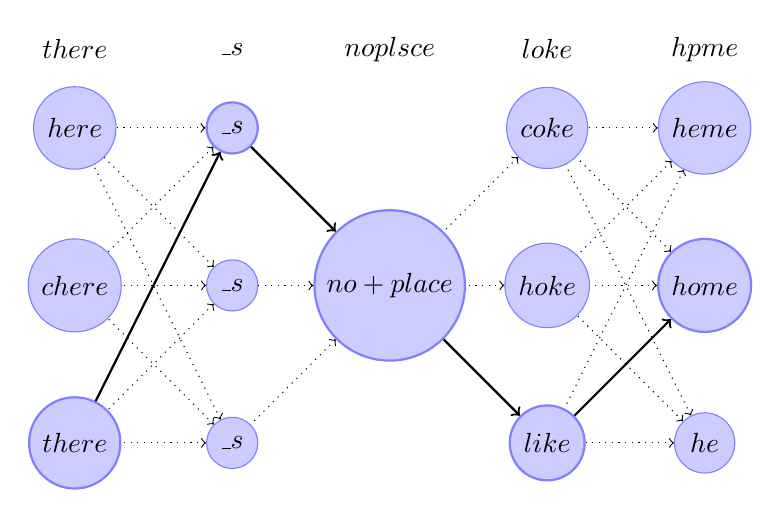
\begin{tikzpicture}[]
% 1st column
\node               at (0,6) {$there$};
\node[state] (s1_1) at (0,5) {$here$};
\node[state] (s2_1) at (0,3) {$chere$};
\node[mainstate] (s3_1) at (0,1) {$there$};
% 2nd column
\node               at (2,6) {$\_s$};
\node[mainstate] (s1_2) at (2,5) {$\_s$}
    edge[lightedge] (s1_1)
    edge[lightedge] (s2_1)
    edge[mainedge] (s3_1);
\node[state] (s2_2) at (2,3) {$\_s$}
    edge[lightedge] (s1_1)
    edge[lightedge] (s2_1)
    edge[lightedge] (s3_1);
\node[state] (s3_2) at (2,1) {$\_s$}
    edge[lightedge] (s1_1)
    edge[lightedge] (s2_1)
    edge[lightedge] (s3_1);
% 3rd column
\node               at (4,6) {$noplsce$};
\node[mainstate] (s2_3) at (4,3) {$no+place$}
    edge[mainedge] (s1_2)
    edge[lightedge] (s2_2)
    edge[lightedge] (s3_2);

% 4th column
\node               at (6,6) {$loke$};
\node[state] (s4_1) at (6,5) {$coke$}
    edge[lightedge] (s2_3);
\node[state] (s4_2) at (6,3) {$hoke$}
    edge[lightedge] (s2_3);
\node[mainstate] (s4_3) at (6,1) {$like$}
    edge[mainedge] (s2_3);
    
% 5th column
\node               at (8,6) {$hpme$};
\node[state] (s5_2) at (8,5) {$heme$}
    edge[lightedge] (s4_1)
    edge[lightedge] (s4_2)
    edge[lightedge] (s4_3);
\node[mainstate] (s2_2) at (8,3) {$home$}
    edge[lightedge] (s4_1)
    edge[lightedge] (s4_2)
    edge[mainedge] (s4_3);
\node[state] (s3_2) at (8,1) {$he$}
    edge[lightedge] (s4_1)
    edge[lightedge] (s4_2)
    edge[lightedge] (s4_3);

\end{tikzpicture}

\end{figure}


e concludendo con la tabella di probabilit\`a ad essa relativa:

\begin{table}[H]
  \centering
  \begin{tabular}{|c|c|c|c|c|}
    \hline
    -12.71720564 & \textbf{-12.79279799} & \textbf{-22.79630544} & -41.38889364 & -62.02404146 \\
    -27.2382859 & -12.79279799 & ... & -42.83453579 & \textbf{-58.53913481} \\
    \textbf{-10.48440738} & -12.79279799 & ... & \textbf{-40.16889086} & -59.36092873 \\
    \hline
  \end{tabular}
\end{table}

\


\subsection{Layered Custom Viterbi}
L'algoritmo appena descritto, cos\`i come il classico algoritmo di 
Viterbi, viene eseguito alla fine valutando tutta la frase nella sua 
interezza e per tale motivo \`e ottimo in fase di testing. 
Tuttavia per una applicazione a run-time quale, ad esempio, una 
tastiera con correttore non si comporta in maniera ottimale, in 
quanto l'esecuzione risulta molto rallentata. 

Per ovviare a questo inconveniente abbiamo sviluppato una versione 
a \textit{layer} per la costruzione della matrice di Viterbi. 
Ovvero una volta inserita la prima parola della frase 
viene costruita la prima colonna
della matrice con le probabilit\`a a priori, mentre all'inserimento 
di ogni altra parola viene valutata ed aggiunta la colonna relativa
alla parola digitata come descritto in ~\ref{sec:vitello}.

Questa particolare versione dell'algoritmo ci ha permesso anche 
di introdurre una caratteristica molto importante ed utile nell'
interfaccia, ovvero la possibilit\`a di suggerire all'utente
tre possibili alternative di correzione, che se verranno confermate
cambieranno le probabilit\`a della matrice di Viterbi di conseguenza.

